\begin{abcliste}
\abc Aus dem Bild liest man die Tabelle ab:
\begin{center}
\begin{tabular}{l|cccccc}
$t$ in \si{\second} & $0$ & $1$ & $2$ & $3$ & $4$ & $5$ \\
\hline
$s$ in \si{\meter} & $0$ & $2.5$ & $4$ & $4.5$ & $4$ & $2.5$ \\
\hline
$\Delta s$ in \si{\meter} & & $2.5$ & $1.5$ & $0.5$ & $-0.5$ & $-1.5$
\end{tabular}
\end{center}
Der Ort nimmt zuerst immer langsamer zu und danach immer schneller ab. Der Graph ist eine $\result{\text{nach unten gekrümmte Kurve (Parabel) mit Maximum bei } t = \tTurnP{0}{1}}$:
\begin{center}
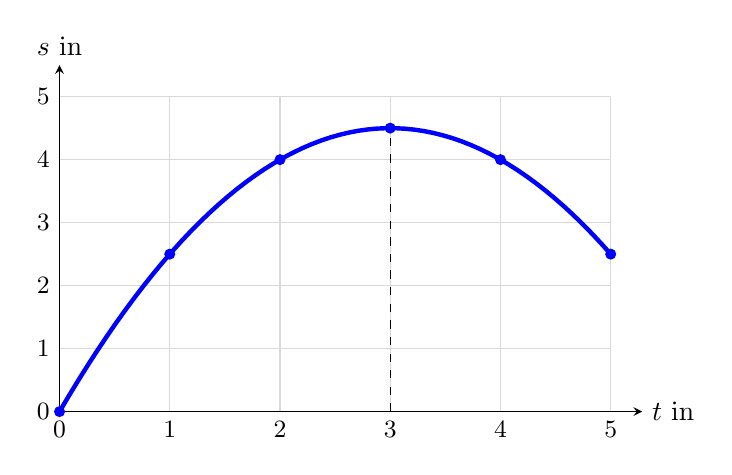
\begin{tikzpicture}[>=stealth, x=1.4cm, y=0.8cm]
 \draw[gray!30] (0,0) grid[xstep=1, ystep=1] (5,5);
 \draw[->] (0,0) -- (5.286,0) node[right] {$t$ in \si{\second}};
 \draw[->] (0,0) -- (0,5.5) node[above] {$s$ in \si{\meter}};
 \foreach \tk in {0,1,2,3,4,5} \node[below] at (\tk,0) {\small $\tk$};
 \foreach \yk in {0,1,2,3,4,5} \node[left] at (0,\yk) {\small $\yk$};

 \draw[ultra thick, blue, domain=0:5, samples=60] plot (\x, {3*\x-0.5*\x*\x});
 \draw[dashed] (3,0) -- (3,4.5);
 \fill[blue] (0,0) circle (2pt);
 \fill[blue] (1,2.5) circle (2pt);
 \fill[blue] (2,4) circle (2pt);
 \fill[blue] (3,4.5) circle (2pt);
 \fill[blue] (4,4) circle (2pt);
 \fill[blue] (5,2.5) circle (2pt);
\end{tikzpicture}
\end{center}
\abc Der Wagen ist bei $t = \tTurnP{0}{1}$ am weitesten vorne, bei $s = \sTurnO$. Davor wird $s$ grösser, danach kleiner: Er $\result{\text{kehrt bei } t = \tTurnP{0}{1} \text{ und } s = \sTurnO \text{ um}}$. Weil die Bilder von \SI{2}{\second} und \SI{4}{\second} (und von \SI{1}{\second} und \SI{5}{\second}) zusammenfallen, liegt der Umkehrpunkt zeitlich genau in der Mitte. In diesem Moment ist die Geschwindigkeit $\result{v = 0}$: Der $s(t)$-Graph hat dort eine waagrechte Tangente.

\abc Die Strecken in aufeinanderfolgenden Sekunden ($2.5$, $1.5$, $0.5$, $-0.5$, $-1.5$ in \si{\meter}) nehmen jedes Mal um denselben Betrag \SI{1}{\meter} ab. Die Geschwindigkeit nimmt also gleichmässig ab: Die Bewegung ist gleichmässig beschleunigt, mit
\begin{align}
 a &= \accF = \frac{\dsTwo-\dsOne}{\left(\dT\right)^2} = \acc \approx \result{\accP{0}{1}}
\end{align}
Das negative Vorzeichen bedeutet: Die Beschleunigung zeigt in die negative Richtung, auch nach dem Umkehren, wenn der Wagen schneller wird.
\end{abcliste}
